\documentclass[12pt]{article}

% Packages
\usepackage[margin=1in]{geometry}
\usepackage{fancyhdr}
\usepackage{amsmath, amsthm, amssymb, physics, graphicx}

% Page Style
\fancypagestyle{plain}{
    \fancyhf{}
    \renewcommand{\headrulewidth}{0pt}
    \renewcommand{\footrulewidth}{0pt}
    \fancyfoot[R]{\thepage}
}
\pagestyle{plain}

% Problem Box
\setlength{\fboxsep}{4pt}
\newsavebox{\savefullbox}
\newenvironment{fullbox}{\begin{lrbox}{\savefullbox}\begin{minipage}{\dimexpr\textwidth-2\fboxsep\relax}}{\end{minipage}\end{lrbox}\begin{center}\framebox[\textwidth]{\usebox{\savefullbox}}\end{center}}
\newenvironment{pbox}[1][]{\begin{fullbox}\ifx#1\empty\else\paragraph{#1}\fi}{\end{fullbox}}

% Options
\renewcommand{\thesubsection}{\thesection(\alph{subsection})}
\allowdisplaybreaks
%\addtolength{\jot}{4pt}
\theoremstyle{definition}

% Default Commands
\newtheorem{proposition}{Proposition}
\newtheorem{lemma}{Lemma}
\newcommand{\ds}{\displaystyle}
\newcommand{\isp}[1]{\quad\text{#1}\quad}
\newcommand{\N}{\mathbb{N}}
\newcommand{\Z}{\mathbb{Z}}
\newcommand{\Q}{\mathbb{Q}}
\newcommand{\R}{\mathbb{R}}
\newcommand{\C}{\mathbb{C}}
\newcommand{\eps}{\varepsilon}
\renewcommand{\phi}{\varphi}
\renewcommand{\emptyset}{\varnothing}
\newcommand{\pfrac}[2]{\left(\frac{#1}{#2}\right)}

% Extra Commands


% Document Info
\fancypagestyle{title}{
    \renewcommand{\headrulewidth}{0.4pt}
    \setlength{\headheight}{15pt}
    \fancyhead[R]{Harry Coleman}
    \fancyhead[L]{GEOG 191 Assignment 7}
    \fancyhead[C]{February 22, 2021}
}

% Begin Document
\begin{document}
\thispagestyle{title}


\begin{pbox}[1]
    Solve using the branch and bound method.
    \[\begin{array}{ll}
        \textbf{Maximize} & z = 5x_1 + 2x_2 \\
        \textbf{Subject to} & 3x_1 + x_2 \leq 12 \\
            & x_1 + x_2 \leq 5 \\
            & x_1, x_2 \geq 0 \\
            & x_1, x_2 \text{ integer}
    \end{array}\]
\end{pbox}

We first relax the integer constraint and solve the linear program.
\begin{center}
    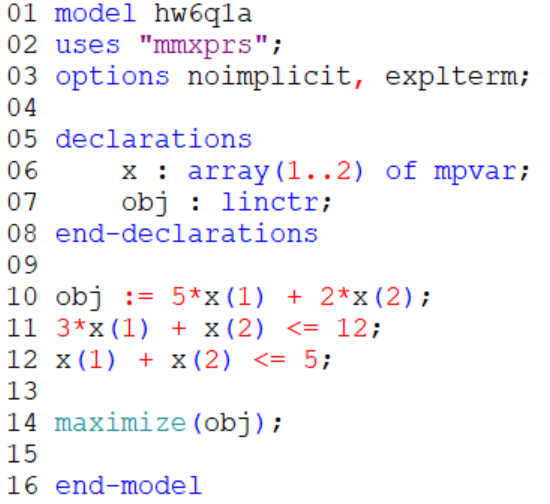
\includegraphics[width=0.4\textwidth]{code1a.png}
    \begin{align*}
        z &= 20.5 \\
        x_1 &= 3.5 \\
        x_2 &= 2.5
    \end{align*}
\end{center}
This result means $20.5$ is an upper bound for the integer program objective. We now make branches for both $x_1 \leq 3$ and $x_1 \geq 4$.
\begin{center}
    \begin{minipage}{0.4\textwidth}
        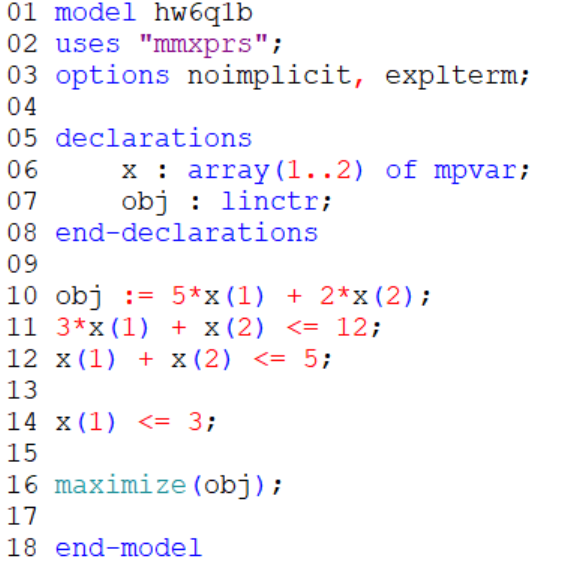
\includegraphics[width=\textwidth]{code1b.png}
        \begin{align*}
            z &= 19 \\
            x_1 &= 3 \\
            x_2 &= 2
        \end{align*}
    \end{minipage}
    \begin{minipage}{0.4\textwidth}
        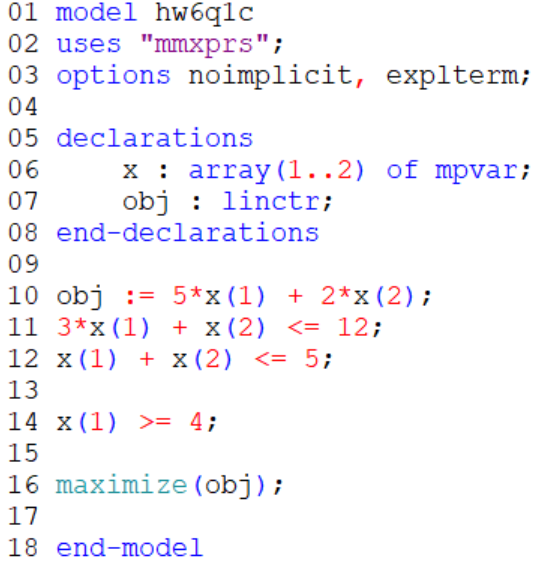
\includegraphics[width=\textwidth]{code1c.png}
        \begin{align*}
            z &= 20 \\
            x_1 &= 4 \\
            x_2 &= 0
        \end{align*}
    \end{minipage}
\end{center}
Both branches have terminated with integer solutions. However, the second branch gives us a better objective. So the optimal solution for the integer program is
\begin{align*}
    z &= 20, \\
    x_1 &= 4, \\
    x_2 &= 0.
\end{align*}



\newpage
\begin{pbox}[3]
    Solve using the branch and bound method.
    \[\begin{array}{ll}
        \textbf{Minimize} & z = 4x_1 + 5x_2 \\
        \textbf{Subject to} & x_1 + 4x_2 \geq 5 \\
            & 3x_1 + 2x_2 \geq 7 \\
            & x_1, x_2 \geq 0 \\
            & x_1, x_2 \text{ integer}
    \end{array}\]
\end{pbox}

We first relax the integer constraint and solve the linear program.
\begin{center}
    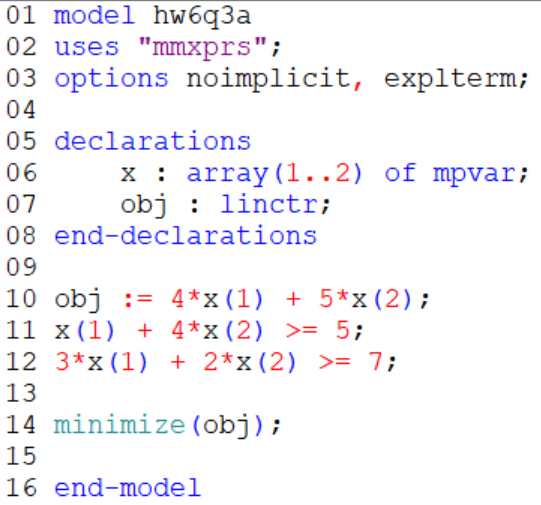
\includegraphics[width=0.4\textwidth]{code3a.png}
    \begin{align*}
        z &= 11.2 \\
        x_1 &= 1.8 \\
        x_2 &= 0.8
    \end{align*}
\end{center}
We now make branches for $x_1 \leq 1$ and $x_1 \geq 2$.
\begin{center}
    \begin{minipage}{0.4\textwidth}
        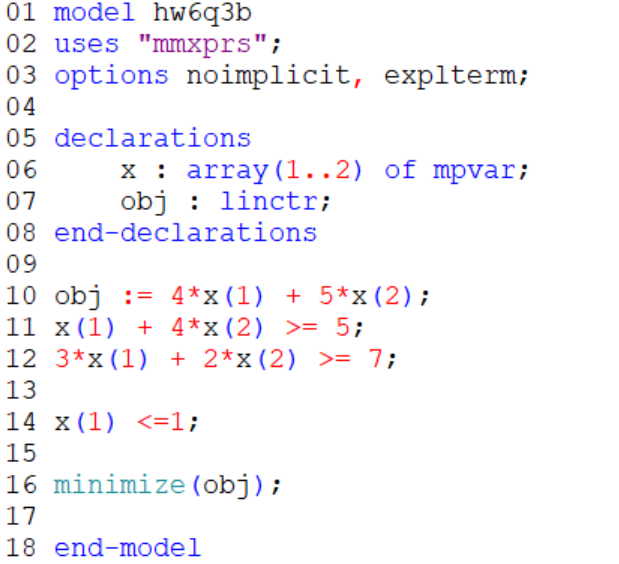
\includegraphics[width=\textwidth]{code3b.png}
        \begin{align*}
            z &= 14 \\
            x_1 &= 1 \\
            x_2 &= 2
        \end{align*}
    \end{minipage}
    \begin{minipage}{0.4\textwidth}
        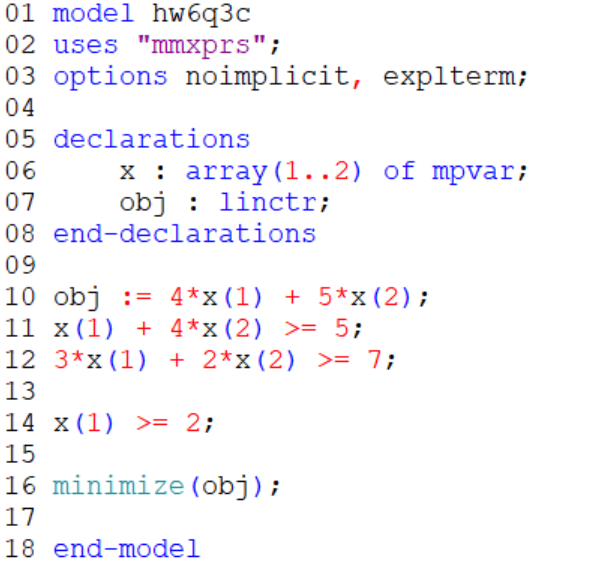
\includegraphics[width=\textwidth]{code3c.png}
        \begin{align*}
            z &= 11.75 \\
            x_1 &= 2 \\
            x_2 &= 0.75
        \end{align*}
    \end{minipage}
\end{center}
The first branch terminates with an integer solution with an objective value of $14$. The second branch gives a rational solution, but it gives a better lower bound on the objective value, $11.75$, so we now make branches for $x_2 \leq 0$ and $x_2 \geq 1$.
\begin{center}
    \begin{minipage}{0.4\textwidth}
        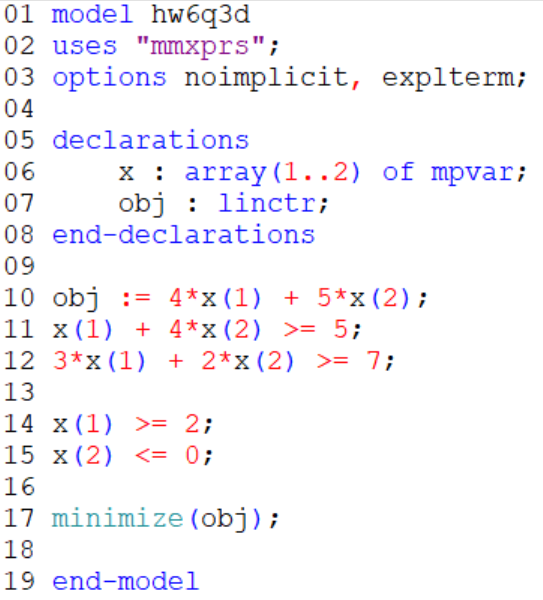
\includegraphics[width=\textwidth]{code3d.png}
        \begin{align*}
            z &= 20 \\
            x_1 &= 5 \\
            x_2 &= 0
        \end{align*}
    \end{minipage}
    \begin{minipage}{0.4\textwidth}
        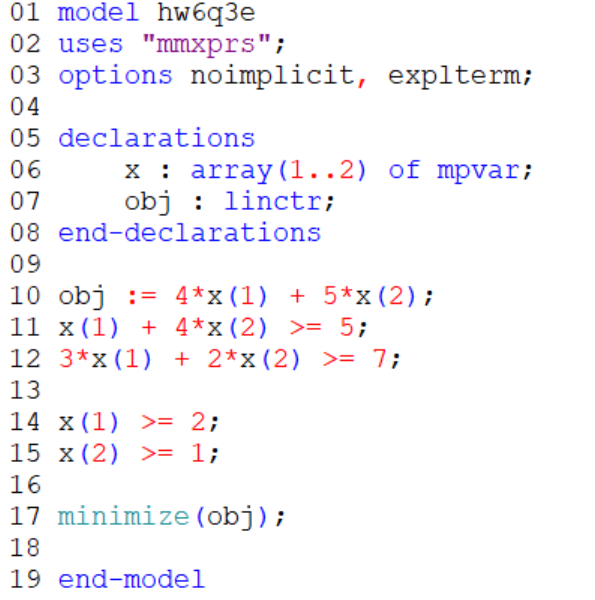
\includegraphics[width=\textwidth]{code3e.png}
        \begin{align*}
            z &= 13 \\
            x_1 &= 2 \\
            x_2 &= 1
        \end{align*}
    \end{minipage}
\end{center}
Both branches terminate with integer solutions. However, the second branch gives a better objective value. So the optimal solution for the integer program is
\begin{align*}
    z &= 13, \\
    x_1 &= 2, \\
    x_2 &= 1.
\end{align*}


\end{document}